
%(BEGIN_QUESTION)
% Copyright 2006, Tony R. Kuphaldt, released under the Creative Commons Attribution License (v 1.0)
% This means you may do almost anything with this work of mine, so long as you give me proper credit

En enhet som kalles et \textit{manometer} er et veldig enkelt, men samtidig veldig nøyaktig instrument for trykkmåling.  Det virker etter prinsippet om at et differansetrykk forskyver en vertikal væskesøyle.  Avstanden mellom toppene av de to væskesøylene er proporsjonal med forskjellen i trykk som legges på toppen av de to vertikale rørene.  Herfra får vi trykkenhetene ``tommer/centimeter vannsøyle'' og ``tommer/centimeter/millimeter kvikksølv'' -- fra hvordan et manometer fungerer:

$$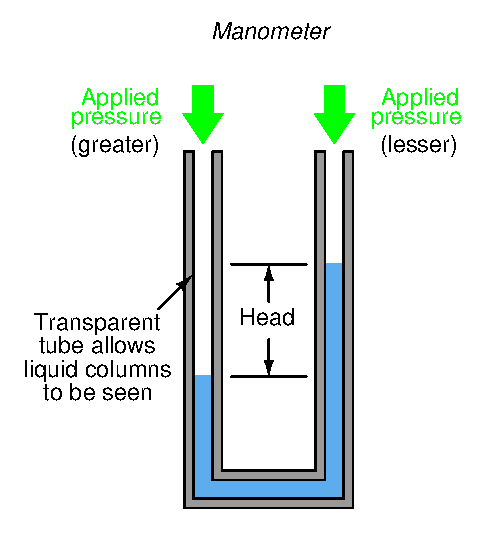
\includegraphics[width=15.5cm]{i00160x01.eps}$$

Forklar hvordan dette instrumentet kan fungere som en standard for trykkmåling, på samme måte som en deadweight-tester kan fungere som standard for trykkgenerering.  Formulert negativt: hva måtte endres for å påvirke målenøyaktigheten til et manometer?

\underbar{file i00160}
%(END_QUESTION)





%(BEGIN_ANSWER)

Noyaktigheten til et manometer bestemmes av to grunnleggende variabler, og begge er ganske konstante:

\begin{itemize}
\item{} Tettheten (masse per volumenhet) til manometervæsken
\item{} Jordens tyngdekraft
\end{itemize}

Så lenge disse to variablene ikke endres, vil heller ikke nøyaktigheten til manometeret endres.

%(END_ANSWER)





%(BEGIN_NOTES)

Så lenge disse to variablene ikke endres, vil heller ikke nøyaktigheten til manometeret endres.  Av disse to er det mest sannsynlig at væskens tetthet endres, og da på grunn av temperaturendring og/eller forurensning.  Så lenge manometeret holdes ved noenlunde konstant romtemperatur, og væsken holdes fri for urenheter, bør manometeret være meget nøyaktig.  Som deadweight-testere og andre instrumenter som avhenger av jordens tyngdekraft, må manometre holdes så nær perfekt vertikal stilling som mulig for å være nøyaktige.

%INDEX% Measurement, pressure: manometer

%(END_NOTES)

